\documentclass[conference]{IEEEtran}
\IEEEoverridecommandlockouts

% Double-blind review: keep true until camera-ready.
\newif\ifanonymous
\anonymoustrue

\usepackage{iftex}
\ifPDFTeX % Overleaf / pdflatex; Tectonic (XeTeX) handles UTF-8 and fonts natively
\usepackage[utf8]{inputenc}
\usepackage[T1]{fontenc}
\fi
\usepackage{amsmath,amssymb}
\ifXeTeX % IEEE requires Times; pdflatex gets it from IEEEtran, XeTeX needs it set
\usepackage{fontspec}
\setmainfont{texgyretermes}[Extension=.otf, UprightFont=*-regular, BoldFont=*-bold,
  ItalicFont=*-italic, BoldItalicFont=*-bolditalic]
\fi
\usepackage{cite}
\usepackage{graphicx}
\usepackage{booktabs}
\usepackage{multirow}
\usepackage{xcolor}
\usepackage{url}
\usepackage[draft]{hyperref} % EDAS rejects PDF links and bookmarks

% Paper-style figures go in figures/; fall back to the project's result figures until then.
\graphicspath{{figures/}{../results/figures/}}

% Drafting aid: \placeholder{...} prints red text. Remove every use before submission.
\newcommand{\placeholder}[1]{\textcolor{red}{[#1]}}

% Keep PDF metadata anonymous.
\hypersetup{pdfauthor={}, pdftitle={}, pdfsubject={}, pdfkeywords={}}

\begin{document}

\title{Who's Actually Answering? Stress-Testing LLM\\Model-Substitution Auditors Against an Adversarial Gateway}

\ifanonymous
\author{\IEEEauthorblockN{Anonymous Author(s)}
\IEEEauthorblockA{Submitted for double-blind review}}
\else
\author{\IEEEauthorblockN{Author Name}
\IEEEauthorblockA{Affiliation\\Email}}
\fi

\maketitle

\begin{abstract}
\placeholder{Abstract, about 150 words. Written last.}
\end{abstract}

\section{Introduction and Threat Model}\label{sec:intro}
A client of an LLM API names a model, pays that model's per-token price, and gets back text along
with a response that repeats the model's name. The repeated name proves nothing. A gateway,
reseller or router between the client and the provider can serve a smaller model, a quantised
copy, or a mix of the two, and still return the name the client asked for. The incentive is large.
For the token mix used in this paper the substitute costs 11.5\% of the genuine model, so a gateway
that swaps one request in ten saves about \$88 per \$1,000 of billed traffic.

The client pays for model $M$, and the only record of what actually ran is the gateway's own. A
provider could attest to the computation in trusted hardware~\cite{cai2025}, but gateways do not
offer this today, and the client has no way to inspect them. What the client can do is test the
responses. A black-box \emph{auditor} sends probe requests and decides, from the text, timing and
metadata that come back, whether the advertised model answered.

At least eight such auditors have appeared since April
2025~\cite{cai2025,zhu2025rut,lin2026gatescope,fang2026kbf,bruckner2026,iris2026,difr2025}. Each
was evaluated on its own testbed and against its own adversary, usually with thresholds chosen on
the same data it reports. A frozen-threshold replication~\cite{holdout2026} shows how fragile this
is: a method with perfect development accuracy fell to 50\% sensitivity on fresh model pairs, and
half of those pairs could not be scored at all. The auditors have never been compared on a common
testbed against a common adversary, and none has been tested against a gateway that expects to be
audited.

\textbf{Threat model.} The client sends requests over HTTPS to a gateway that advertises model $M$.
The gateway controls routing and response metadata. For each request it may forward to $M$, to a
cheaper substitute $M'$, to another provider of $M$, or to a cache. It may rewrite the reported
model name, the \texttt{usage} token counts and \texttt{system\_fingerprint}, and it may add delay.
Because it reads every request, it can classify requests by their shape. It does not know a given
auditor's probes or thresholds, but it knows the published methods and the public benchmarks. Its
goal is to save as much as possible while keeping the probability of detection low. The client
sees only what crosses the wire: response text, client-side latency, the \texttt{usage} block, the
fingerprint, and logprobs where the endpoint exposes them. Timing is a side channel the client can
measure without the gateway's cooperation; content is the only other signal. Honest variation, such
as load balancing across legitimate providers of $M$, is permitted and must not be flagged.

\textbf{Contributions.}
\begin{itemize}
\item \textbf{A shared adversarial testbed.} SHIM is an OpenAI-compatible gateway with twelve
  adversary arms and a hidden ledger of which backend really answered. Four of the arms
  (probe-aware evasion, laundering, canary-awareness and benign routing) appear in no prior
  evaluation.
\item \textbf{A sealed comparison of six auditors.} We reimplement five published methods and add an
  e-value fusion, all evaluated under thresholds hashed and tagged before evaluation. An auditor
  that cannot run reports \emph{uninformative}, never \emph{pass}.
\item \textbf{Deployability on real endpoints.} On 11 free-tier endpoints, a logprob-based auditor
  runs on none and the one-token method as published on 4, because hidden reasoning tokens use up
  its token budget.
\item \textbf{Three negative results.} Probe-aware evasion keeps every auditor at chance.
  False-positive budgets, not audit cost, set a dilution floor of $\epsilon^* \approx 0.10$. Timing
  auditors cannot tell fraud from sanctioned routing, which splits ``substitution'' into identity,
  disclosure and billing violations.
\end{itemize}

% Converted from drafts/02_related.md. Budget: 0.5 pages.
\section{Related Work}\label{sec:related}
\placeholder{Related Work: 0.5 pages.}

% Converted from drafts/03_design.md. Budget: 1.0 page.
\section{System Design}\label{sec:design}

The testbed has two parts: SHIM, a gateway that cheats in controlled ways, and ARENA, which runs
auditors against it under a sealed protocol.

\textbf{SHIM.} SHIM is an HTTP server that implements the OpenAI chat-completions API, including
the \texttt{usage} block and \texttt{system\_fingerprint}. An auditor points its base URL at SHIM
and cannot distinguish it from a provider except by behaviour. Each request passes through one of
twelve \emph{adversary arms} (Table~\ref{tab:arms}), which decide which backend answers and how the
response is rewritten. Randomised arms seed on a hash of the request body, never on wall-clock
time, so every run replays exactly. For every request SHIM appends a ledger line recording the arm,
the backend that really answered, latency, reported and true token usage, and imputed cost from
public price tables. No auditor can read the ledger. It is the ground truth from which every ROC
curve and false-positive rate in this paper is computed, which no audit of a real gateway can do.

\begin{table}[t]
\centering
\caption{Adversary arms. Bold arms appear in no prior evaluation. A4 and A11 serve the genuine
model and test specificity.}
\label{tab:arms}
\small
\begin{tabular}{@{}llc@{}}
\toprule
Arm & Gateway behaviour & Truth \\
\midrule
A0 & Honest & genuine \\
A1 & Always serves the substitute & subst. \\
A2 & Same model name, other provider & subst. \\
A3 & Substitute on a fraction $\epsilon$ of requests & subst. \\
A4 & Right model, altered sampling settings & genuine \\
\textbf{A5} & Honest only on audit-shaped requests & subst. \\
A6 & Replays cached answers to repeated prompts & subst. \\
\textbf{A7} & Substitute answers, second pass restyles & subst. \\
A8 & Inflates reported token usage & subst. \\
A9 & Adds delay to mimic the genuine latency & subst. \\
\textbf{A10} & Honest on public benchmark questions & subst. \\
\textbf{A11} & Splits traffic across honest providers of $M$ & genuine \\
\bottomrule
\end{tabular}
\end{table}

Three arms deserve detail. \textbf{A5} (probe-aware evasion) routes a request to the genuine model
when it \emph{looks like an audit}: at most 24 \texttt{max\_tokens}, a prompt under 220 characters,
a prompt seen before, or a closed-answer phrase such as ``reply with only''. It needs no knowledge
of any particular probe set, only of the shape that cheap probes share. \textbf{A10} keeps a static
list of public benchmark questions and answers those honestly. \textbf{A11} is not an attack: it
spreads traffic across legitimate providers of the correct model, as commercial routers do by
default~\cite{openrouter_exacto}, and is scored as a false-positive test.

Backends are either a \emph{replay corpus} of real responses, recorded once from free-tier endpoints
and committed so that every auditor sees byte-identical data, or a \emph{mock} whose model
personalities (answer preferences, surface habits, accuracy, latency) can be sampled in unlimited
sessions. We use two mock ladders: one hand-written, and one whose answer distributions and latency
are fitted to the recorded census and the live run (Section~\ref{sec:results}).

\textbf{ARENA.} Six auditors implement one interface that returns a score, a p-value and an
\texttt{applicable} flag (Table~\ref{tab:auditors}). Five are reimplementations labelled
\emph{-lite}, since none is the authors' code. FUSE is new: it converts each applicable auditor's
calibrated p-value to an e-value, multiplies them, and flags when the product exceeds $1/\alpha$,
which by Ville's inequality controls the Type-I error at any stopping
time~\cite{vovk2021evalues,ville1939}.

\begin{table}[t]
\centering
\caption{Auditors. Five reimplementations and one new fusion.}
\label{tab:auditors}
\small
\setlength{\tabcolsep}{4pt}
\begin{tabular}{@{}lll@{}}
\toprule
Auditor & Source & Signal \\
\midrule
OTE & \cite{bruckner2026} & JSD of single-answer distributions, 8 cells \\
IRIS-lite & \cite{iris2026} & 16 surface-string features, random forest \\
GATEOPS & \cite{lin2026gatescope} & latency KS test, fingerprint, billing \\
KBF & \cite{fang2026kbf} & agreement on 15 knowledge-boundary facts \\
BENCH & \cite{cai2025} & accuracy on 12 MMLU/GPQA/GSM8K items \\
RUT & \cite{zhu2025rut} & token-rank uniformity (needs logprobs) \\
FUSE & new & product of e-values, flag at $E > 1/\alpha$ \\
\bottomrule
\end{tabular}
\end{table}

\textbf{Sealed protocol.} A session is one audit of 495 queries. Each threshold is the largest
score seen over $N$ honest (A0) calibration sessions, which bounds the marginal false-positive rate
by $1/(N+1)$; a session is flagged when its score \emph{strictly} exceeds the threshold. With
$\alpha = 0.01$ and $N = 300$, the realised false-positive rate exceeds $\alpha$ with probability at
most $0.99^{300} = 4.9\%$. The thresholds and all decision rules are written to one file, hashed
with SHA-256, committed and tagged before any evaluation runs, and every evaluation script refuses
to run if the hash has changed. An auditor that cannot run on an endpoint, or on a response without
the field it needs, returns \emph{uninformative}, never \emph{consistent}. Our first seal (v1,
$N = 100$) used a $\ge$ rule; we report its results as sealed and correct the rule in a second seal
(v2) rather than editing v1.

% Converted from drafts/04_results.md. Budget: 1.75 pages.
\section{Results}\label{sec:results}
\placeholder{Results: 1.75 pages.}

% Converted from drafts/05_economics.md. Budget: 1.0 page.
\section{Economics and the Routing Confound}\label{sec:econ}

\textbf{Break-even.} At dilution rate $\epsilon$ the gateway saves
$\$1{,}000 \cdot \epsilon \cdot (1 - r)$ per \$1,000 of billed traffic, where $r = 0.115$ is the
price ratio of substitute to genuine model. Against this we set the imputed cost of enough audit
sessions to reach 80\% detection power, using measured token counts and public list prices. Both
curves are shown in Fig.~\ref{fig:F2}.

\begin{figure}[t]
\centering
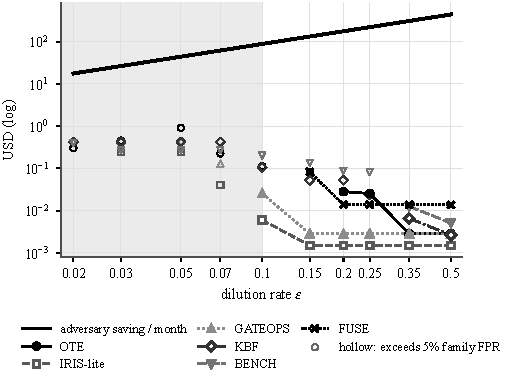
\includegraphics[width=\columnwidth]{fig_break_even}
\caption{Break-even (v2, hand-written ladder). Adversary saving per \$1,000 of monthly traffic vs.\
imputed cost of an audit reaching 80\% power, by dilution rate. Hollow markers exceed the 5\%
family false-positive budget. No admissible audit exists left of $\epsilon^*$ (shaded).}
\label{fig:F2}
\end{figure}

Cost is never the obstacle. One audit session costs between \$0.0013 (KBF) and \$0.014 (FUSE), and
wherever an auditor reaches 80\% power the total is below one cent, against savings of tens of
dollars. On price alone, auditing always pays.

False positives are the obstacle. Repeating a session raises power, but it raises false alarms
too: with per-session false-positive rate $f$, $k$ sessions raise at least one false alarm with
probability $1 - (1-f)^k$. The protocol seals a family budget of 5\%, which caps each auditor at 6
to 15 sessions. Below $\epsilon = 0.10$ per-session power collapses: at $\epsilon = 0.07$ the best
auditor detects 6\% of sessions on the hand-written ladder and 1\% on the fitted one, so no
admissible number of repeats reaches 80\%. The smallest dilution an admissible audit detects is
therefore $\epsilon^* = 0.10$ on both ladders, with a bootstrap 95\% interval of [0.10, 0.10].
IRIS-lite gets there with 34\% power per session and 4 sessions (hand-written ladder) or 56\% and 2
sessions (fitted ladder), for \$0.003--\$0.006.

One caveat changes the number. IRIS-lite sets $\epsilon^*$ on both ladders, but on real recordings
its features cannot separate 20b from 120b (Section~\ref{sec:real}); its mock signal comes from
hand-written surface habits. Removing it after the seal, as a post-hoc and unsealed check, leaves
$\epsilon^* = 0.10$ on the hand-written ladder and moves it to $0.15$ on the fitted ladder, both set
by GATEOPS. We therefore claim $\epsilon^* \in [0.10, 0.15]$. A rational gateway sets $\epsilon$
just below it. At $\epsilon = 0.05$ it still saves \$44 per \$1,000, and no auditor here detects it
within a false-alarm budget a customer would accept.

\textbf{The confound.} A3 at $\epsilon = 0.10$ sends 10\% of traffic to a cheaper model. A11
spreads traffic across honest providers of the correct model. The first is fraud; the second is
ordinary load balancing, and routers do it by default. Fig.~\ref{fig:F6} and
Table~\ref{tab:confound} compare them over 200 sessions each.

\begin{figure}[t]
\centering
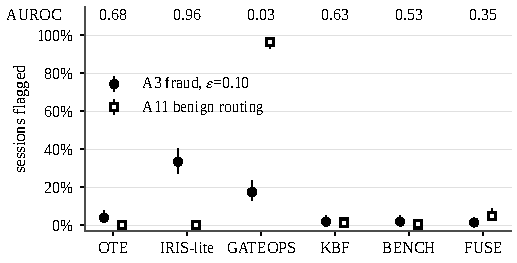
\includegraphics[width=\columnwidth]{fig_confound}
\caption{Share of sessions flagged, A3 (fraud, $\epsilon = 0.10$) vs.\ A11 (benign routing), v2
hand-written ladder, 200 sessions each. Top row: AUROC of A3 vs.\ A11. Timing-based scores rank
benign routing above fraud.}
\label{fig:F6}
\end{figure}

\begin{table}[t]
\centering
\caption{A3 ($\epsilon = 0.10$, fraud) vs.\ A11 (benign routing), hand-written / fitted ladder.
AUROC below 0.5 means benign routing scores as more suspicious than fraud.}
\label{tab:confound}
\small
\setlength{\tabcolsep}{4pt}
\begin{tabular}{@{}lccc@{}}
\toprule
Auditor & Flags A3 & Flags A11 & AUROC \\
\midrule
IRIS-lite & 34\% / 56\% & 0\% / 0\% & 0.96 / 0.98 \\
OTE & 4\% / 0\% & 0\% / 0\% & 0.68 / 0.48 \\
GATEOPS & 18\% / 5\% & 96\% / 100\% & 0.03 / 0.00 \\
FUSE & 2\% / 0\% & 5\% / 50\% & 0.35 / 0.01 \\
\bottomrule
\end{tabular}
\end{table}

GATEOPS finds benign routing \emph{more} anomalous than fraud (AUROC 0.00--0.03), and FUSE inherits
this: on the fitted ladder it flags half of all honest routing sessions and no fraud sessions.
Timing and metadata measure whether traffic is \emph{heterogeneous}, not whether the model is
\emph{wrong}, and honest routing is maximally heterogeneous. The text auditors separate the two arms
only because our simulated alternate provider returns near-identical text. A real alternate
provider running a different engine or quantisation would shift the text too, and the gap would
narrow.

This suggests that ``model substitution'' merges three violations that need different evidence:
\begin{itemize}
\item \emph{Identity:} the weights are wrong (A1, A2, A7). Content signals can observe this.
\item \emph{Disclosure:} routing happens but is not disclosed (A3 vs.\ A11). The two differ only in
  intent, which no client-side measurement observes.
\item \emph{Billing:} the invoice does not match the service (A8). This needs an invoice, and free
  tiers issue none.
\end{itemize}
Only the first is a detection problem for black-box auditors. The second needs a disclosure
obligation on the gateway, and the third needs verifiable metering. This reaches the recommendation
of hardware attestation in~\cite{cai2025} from the opposite direction: part of what auditors are
asked to detect is not observable from the client at all.

% Converted from drafts/06_conclusion.md. Budget: 0.5 pages.
\section{Limitations and Conclusion}\label{sec:conclusion}
\placeholder{Limitations and Conclusion: 0.5 pages.}

\paragraph{Artifact} The gateway, auditors, sealed protocols, replay corpus and every figure are
available at an anonymised repository:
\url{https://anonymous.4open.science/r/model-substitution-simu-0F5B}. All results except the live
run regenerate without an API key.

% IEEE policy on AI-generated text: name the AI system, the sections it was used in, and the
% extent of use. Keep this section free of names while the submission is anonymous.
\section*{Acknowledgment}
In line with IEEE policy on AI-generated content, we disclose that the text of all sections of
this paper, including the abstract, was drafted by Claude, an AI system developed by Anthropic,
used through Claude Code. The same system also wrote much of the experiment software (the SHIM
gateway, the auditor reimplementations and the analysis scripts) under the authors' direction.
The authors set the research question and the study design, ran the experiments against the
free-tier endpoints, revised the text, and checked every number, citation and figure against the
recorded results and the cited sources. The authors take full responsibility for the content of
this paper.


\bibliographystyle{IEEEtran}
\bibliography{refs}

\end{document}
